%===============================================================================
\documentclass[a4paper]{ifacconf}

% Pacotes Essenciais
\usepackage{graphicx,amsmath,url}
\usepackage[round]{natbib}
\usepackage{xcolor}
\usepackage{float}
\usepackage{subcaption}
\usepackage{circuitikz}
\usepackage{tikz}

% Configuração de Idioma e Codificação
\usepackage[english,brazil]{babel}
\usepackage[T1]{fontenc}
\usepackage[utf8]{inputenc}
\usepackage{ae}

% Definições de Ambientes Matemáticos
\newtheorem{teorema}[thm]{{\em Teorema}}{ }
\newtheorem{lema}[thm]{{\em Lema}}{ }
\newtheorem{corolario}[thm]{{\em Corolário}}{ }
\newenvironment{prova}{{\bf Prova.}}{ }

\begin{document}

\begin{frontmatter}

\title{Desenvolvimento e Controle de Conversor CC-CC de Três Portas Utilizando Técnica FCS-MPC para Sistemas Fotovoltaicos com Armazenamento}

\author[First]{João Vitor Santos Barbosa}
\author[First]{Silvia Costa Ferreira}

\address[First]{Departamento de Automática, Universidade Federal de Lavras, MG.}

% --- RESUMO E ABSTRACT ---
\selectlanguage{english}
\renewcommand{\abstractname}{} % Limpa o título padrão do template para inserirmos manualmente
\begin{abstract}
\selectlanguage{brazil}
{\noindent \bf Resumo}:
A crescente inserção da geração fotovoltaica em micro-redes exige sistemas eficientes de armazenamento e regulação para mitigar a intermitência solar. Este trabalho propõe o desenvolvimento e a simulação computacional de um conversor CC-CC de três portas do tipo VR-BESS (Voltage Regulator - Battery Energy Storage System), a ser controlado pela técnica de Controle Preditivo Baseado em Modelo com Conjunto Finito de Controle (FCS-MPC). A topologia adotada reduz a contagem de componentes ao utilizar um indutor compartilhado e apenas duas chaves semicondutoras para gerenciar o fluxo de potência entre o painel fotovoltaico, o banco de baterias e a carga. A modelagem matemática do sistema foi implementada em ambiente MATLAB/Simulink, combinando funções analíticas no domínio de sinal para a planta fotovoltaica e a bateria de íon-lítio com a simulação física do conversor no Simscape Electrical. Nesta etapa do trabalho, os subsistemas de painel fotovoltaico e banco de baterias, desenvolvidos como blocos mascarados próprios em substituição às bibliotecas nativas do Simscape (indisponíveis no ambiente MATLAB Online utilizado), foram integrados ao conversor VR-BESS e validados em malha aberta, com as chaves operando sob sinais PWM de razão cíclica fixa, recalculada a partir do ponto de operação autoconsistente do arranjo fotovoltaico. Os resultados confirmam a correta integração entre os domínios de sinal e físico do Simscape e a coerência das tensões e do estado de carga observados com os parâmetros de projeto adotados, consolidando a base de simulação sobre a qual o controlador FCS-MPC será implementado e avaliado na próxima etapa do trabalho.

\vskip 3mm
\selectlanguage{english}
{\noindent \bf Abstract}:
The increasing penetration of photovoltaic generation in microgrids requires efficient storage and regulation systems to mitigate solar intermittency. This paper presents the development and computational simulation of a three-port DC-DC converter of the VR-BESS (Voltage Regulator - Battery Energy Storage System) type, to be controlled by the Finite Control Set Model Predictive Control (FCS-MPC) technique. The adopted topology reduces component count by using a shared inductor and only two semiconductor switches to manage the power flow among the photovoltaic panel, the battery bank, and the load. The mathematical modeling of the system was implemented in the MATLAB/Simulink environment, combining analytical functions in the signal domain for the photovoltaic plant and the lithium-ion battery with the physical simulation of the converter in Simscape Electrical. At this stage of the work, the photovoltaic panel and battery bank subsystems, developed as custom masked blocks in place of the native Simscape libraries (unavailable in the MATLAB Online environment used), were integrated with the VR-BESS converter and validated in open loop, with the switches driven by fixed duty-cycle PWM signals recalculated from the self-consistent operating point of the photovoltaic array. Results confirm the correct integration between the signal and physical domains of Simscape and the consistency of the observed voltages and state of charge with the adopted design parameters, consolidating the simulation baseline upon which the FCS-MPC controller will be implemented and evaluated in the next stage of the work.
\end{abstract}

% --- PALAVRAS-CHAVE ---
\begin{keyword}
\selectlanguage{brazil}
{\noindent\it Palavras-chaves:} Controle Preditivo Baseado em Modelo, Conversor de Três Portas, Sistemas Fotovoltaicos, Armazenamento de Energia, FCS-MPC.

\vskip 2mm
\selectlanguage{english}
{\noindent\it Keywords:} Model Predictive Control, Three-Port Converter, Photovoltaic Systems, Energy Storage, FCS-MPC.
\end{keyword}

\selectlanguage{brazil}
\end{frontmatter}

%===============================================================================
% CORPO DO TEXTO
%===============================================================================

\section{Introdução}
\label{sec:introducao}

A crescente penetração da geração fotovoltaica nas redes elétricas tem sido
acompanhada por desafios relacionados à intermitência e à variabilidade
dessa fonte, que comprometem a estabilidade do fornecimento de energia e a
qualidade de tensão em sistemas de pequeno e médio porte
\citep{ayaz2014improved}. Para mitigar esses efeitos, sistemas de
armazenamento de energia em baterias (\textit{Battery Energy Storage
System} -- BESS) têm sido amplamente incorporados a instalações
fotovoltaicas, atuando como reguladores de potência e garantindo o
suprimento contínuo da carga mesmo sob variações bruscas de irradiância.

A integração entre o painel fotovoltaico, o banco de baterias e a carga é
tradicionalmente realizada por meio de conversores CC-CC independentes, um
para cada fonte, conectados a um barramento comum. Essa abordagem, embora
simples, implica maior número de componentes, perdas adicionais de
conversão e custo elevado. Como alternativa, conversores CC-CC de múltiplas
portas têm sido propostos para integrar essas três interfaces em um único
estágio de potência, reduzindo a complexidade do sistema sem comprometer a
flexibilidade no gerenciamento do fluxo de energia \citep{zhang2025adaptive}.

Por outro lado, a operação desses conversores envolve o acoplamento entre
múltiplas portas, incertezas paramétricas e perturbações de carga não
lineares, fatores que reduzem a eficácia de controladores clássicos de
ganho fixo, como o PID, frente a variações bruscas de operação
\citep{zhang2025adaptive}. Técnicas de controle preditivo baseado em modelo
têm-se mostrado uma alternativa robusta para esse cenário, por incorporar
diretamente, na própria formulação do problema de controle, as restrições
físicas do sistema e suas múltiplas variáveis. Dentro dessa classe de
controladores, o Controle Preditivo Baseado em Modelo com Conjunto Finito
de Controle (\textit{Finite Control Set Model Predictive Control} --
FCS-MPC) explora diretamente a natureza discreta dos conversores
eletrônicos de potência, prescindindo da etapa de modulação por largura de
pulso (PWM) e permitindo respostas dinâmicas rápidas mesmo em sistemas
multivariáveis \citep{ferreira2018finite, wang2023fcsmpc}.

Neste trabalho, adota-se a topologia de conversor de três portas do tipo
VR-BESS (\textit{Voltage Regulator -- Battery Energy Storage System}), que
integra a porta fotovoltaica, a porta de armazenamento e a porta de carga
utilizando apenas duas chaves semicondutoras e um indutor compartilhado,
operando como conversor \textit{Buck} durante o carregamento da bateria e
como \textit{Boost} na regulação da tensão de saída. O número reduzido de
chaves resulta em um conjunto de estados de comutação naturalmente pequeno,
o que torna essa topologia particularmente adequada à aplicação direta do
FCS-MPC, cujo custo computacional cresce com o número de estados avaliados
a cada período de amostragem.

O objetivo deste trabalho é desenvolver e simular o controle do conversor
VR-BESS por meio da técnica FCS-MPC, a partir da modelagem em espaço de
estados do conversor e do painel fotovoltaico associado. Além disso, serão
estudados observadores de estado como alternativa para reduzir a
quantidade de sensores físicos necessários à implementação do
controlador, contribuindo para uma solução de controle mais simples e de
menor custo de instrumentação. Como etapa prévia à síntese do controlador,
este trabalho apresenta a modelagem e a validação em malha aberta do
conversor VR-BESS e de seus subsistemas de painel fotovoltaico e banco de
baterias, implementados como bibliotecas próprias no Simscape Electrical.
Essa validação estabelece a base de simulação sobre a qual o controlador
FCS-MPC será desenvolvido e avaliado, em cenários de variação de
irradiância, carga e referência de tensão, na etapa subsequente do
trabalho.

\section{Referencial Teórico}
\label{sec:refteorico}

Esta seção apresenta os conceitos necessários ao desenvolvimento do conversor
CC-CC de três portas controlado pela técnica FCS-MPC: a modelagem de
conversores multiporta, a representação do painel fotovoltaico, os
fundamentos do controle preditivo baseado em modelo com conjunto finito de
controle (FCS-MPC) e os observadores de estado empregados na redução da
instrumentação do sistema.

\subsection{Conversores CC-CC de Três Portas}
\label{subsec:conversor3portas}

Conversores de três portas integram fonte, armazenamento e carga em um único
estágio de potência, reduzindo o número de componentes em relação ao uso de
conversores independentes \citep{zhang2025adaptive}. Na topologia VR-BESS
adotada neste trabalho (Fig.~\ref{fig:topologia}), duas chaves
semicondutoras e um indutor compartilhado regulam o fluxo de potência entre
as portas de geração fotovoltaica, armazenamento (BESS) e carga, operando
como conversor \textit{Buck} durante o carregamento da bateria e como
\textit{Boost} durante a regulação da tensão de saída.

\begin{figure}[h]
\centering
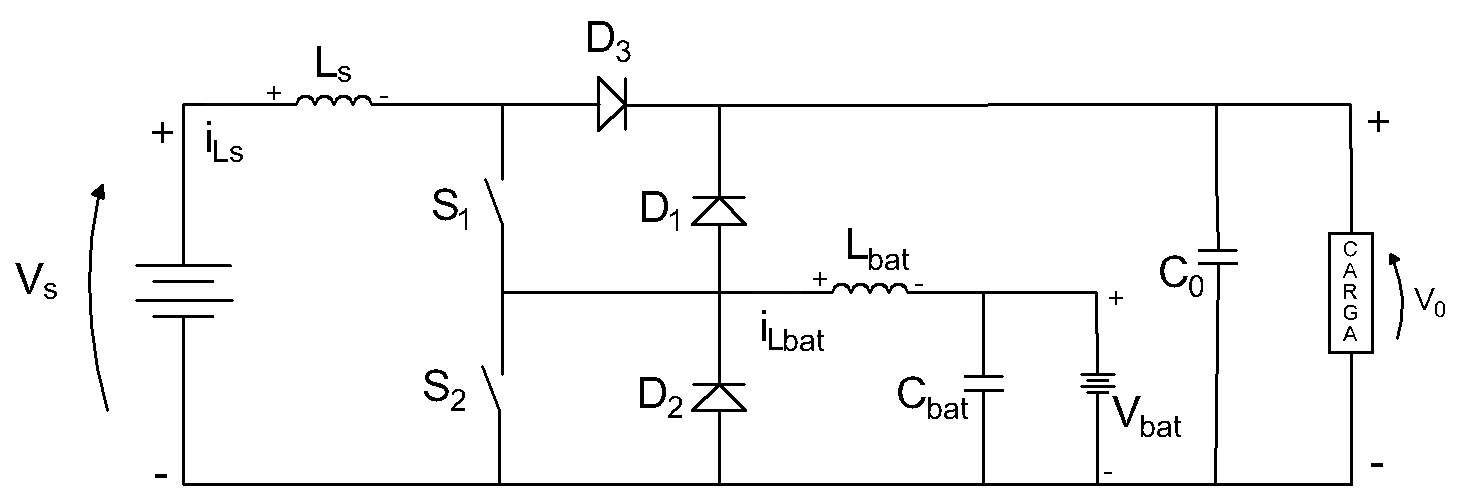
\includegraphics[width=\linewidth]{Figuras/topologia_3portas.png}
\caption{Representação conceitual da topologia de duas chaves do conversor
de três portas (FV--BESS--Carga).}
\label{fig:topologia}
\end{figure}

O modelo de valores médios de cada porta $x$ é obtido a partir do balanço de
carga no respectivo capacitor, podendo ser escrito de forma geral como

\begin{equation}
\dot V_x = \frac{1}{C_x}I_x - \frac{1}{C_x R_x}V_x,
\label{eq:portmodel}
\end{equation}

em que $I_x$ é a corrente injetada na porta, $C_x$ a capacitância
equivalente e $R_x$ a resistência de carga vista por essa porta
\citep{zhang2025adaptive}. A Eq.~\eqref{eq:portmodel}, aplicada a cada porta
do conversor, fundamenta a representação em espaço de estados sobre a qual o
controlador FCS-MPC atua.

\subsection{Modelagem do Painel Fotovoltaico}
\label{subsec:modelopv}

A porta de entrada do conversor é alimentada por um painel FV representado
pelo circuito equivalente de diodo único, cuja corrente de saída é função da
tensão nos terminais:

\begin{equation}
I_y = I_{SC}\left[1 - K_1\!\left(e^{V_y/(K_2 V_{OC})} - 1\right)\right],
\label{eq:pvmodel}
\end{equation}

em que $K_1$ e $K_2$ são obtidos a partir dos parâmetros de catálogo
($I_{SC}$, $I_{MP}$, $V_{OC}$, $V_{MP}$) nas condições padrão de teste
\citep{ayaz2014improved}. Esses parâmetros são corrigidos em função da
irradiância $G$ e da temperatura de célula $T_C$, sendo esta última estimada
a partir da temperatura ambiente, da irradiância e da velocidade do vento. O
modelo, validado experimentalmente para módulos monocristalinos,
policristalinos e de filme fino, apresentou desvios de energia entre $3,25\%$
e $13,93\%$ em relação aos dados medidos \citep{ayaz2014improved}, sendo
adotado neste trabalho para representar a fonte conectada à porta FV do
conversor.

\subsection{Controle Preditivo Baseado em Modelo com Conjunto Finito de Controle (FCS-MPC)}
\label{subsec:fcsmpc}

O FCS-MPC explora o número finito de estados de comutação de um conversor
para, a cada período de amostragem: (i) predizer o valor futuro das
variáveis de estado $x^P(k+1)$ para cada estado de comutação $S_n$
disponível; (ii) avaliar uma função de custo que pondera o erro entre
$x^{P}$ e a referência $x^{*}$; e (iii) aplicar o estado $S_{opt}$ que
minimiza essa função, repetindo o processo no instante seguinte
\citep{ferreira2018finite, wang2023fcsmpc} (Fig.~\ref{fig:fcsmpc}).

\begin{figure}[h]
\centering
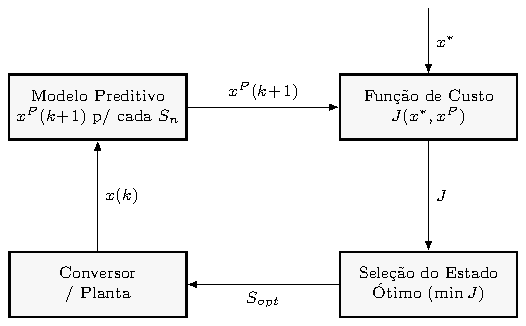
\includegraphics[width=\linewidth]{Figuras/fcsmpc_diagrama.pdf}
\caption{Estrutura genérica do controle FCS-MPC.}
\label{fig:fcsmpc}
\end{figure}

Para conversores com múltiplas variáveis controladas, a função de custo pode
ser definida de forma multivariável, ponderando o erro de cada variável por
um ganho independente, como em

\begin{equation}
J = K_1\left|x_1^{*} - x_1^{P}\right| + K_2\left|x_2^{*} - x_2^{P}\right|,
\label{eq:costfunction}
\end{equation}

em que $K_1$ e $K_2$ definem a prioridade relativa entre os objetivos de
controle \citep{ferreira2018finite}. O principal fator limitante do FCS-MPC é
o crescimento do esforço computacional com o número de estados de comutação
e com o horizonte de predição $N$; em conversores multinível, esse custo
pode ser reduzido por meio de estruturas híbridas que combinam redes
neurais com o próprio FCS-MPC, alcançando reduções de até $58,8\%$ no esforço
computacional \citep{wang2023fcsmpc}. Conversores com poucas chaves, como o
VR-BESS aqui adotado, possuem um conjunto de estados naturalmente reduzido,
o que favorece a aplicação direta do FCS-MPC sem a necessidade dessas
estruturas auxiliares.

\subsection{Observadores de Estado e Controle por Rejeição Ativa de Distúrbios}
\label{subsec:observadores}

Conversores multiporta apresentam acoplamento entre portas e incertezas
paramétricas que limitam o desempenho de controladores de ganho fixo
\citep{zhang2025adaptive}. O controle por rejeição ativa de distúrbios (ADRC)
trata essas incertezas, em conjunto com dinâmicas não modeladas, como um
\textit{distúrbio total}, estimado em tempo real por um observador de
estados estendido (ESO) e compensado na lei de controle.

Para melhorar simultaneamente a imunidade a ruído em regime permanente e o
rastreamento durante transitórios, pode-se empregar um observador
adaptativo (AESO) que alterna entre um observador linear tradicional
(TLESO) e um observador baseado em malha de captura de fase (PLLO),
conforme a Fig.~\ref{fig:aeso}. A comutação é definida por um limiar de erro

\begin{equation}
\mu = \Delta V + \delta,
\label{eq:threshold}
\end{equation}

combinado a temporizadores de confirmação ($t_{1d}$, $t_{2d}$) que evitam
comutações espúrias \citep{zhang2025adaptive}.

\begin{figure}[h]
\centering
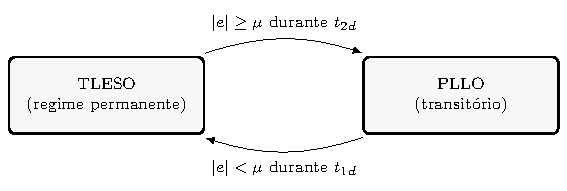
\includegraphics[width=\linewidth]{Figuras/aeso_diagrama.pdf}
\caption{Lógica de comutação entre os observadores TLESO e PLLO.}
\label{fig:aeso}
\end{figure}

Embora o presente trabalho adote o FCS-MPC como estratégia principal de
controle, o uso de observadores de estado é relevante para a etapa de
simulação prevista neste TCC, na qual se pretende avaliar sua aplicação como
alternativa para reduzir o número de sensores físicos necessários à
implementação do controle preditivo no conversor VR-BESS.

\section{Metodologia}
\label{sec:metodologia}

Esta seção descreve os procedimentos adotados na implementação do conversor
VR-BESS e de seus subsistemas (painel fotovoltaico e banco de baterias) em
ambiente MATLAB/Simulink, com os componentes elétricos representados no
domínio físico do Simscape Electrical.

\subsection{Topologia do Conversor Implementada}
\label{subsec:topologia_impl}

A topologia VR-BESS implementada segue a estrutura descrita por
\cite{srinivasa2016vrbess}, composta por dois indutores ($L_s$, $L_{bat}$),
duas chaves semicondutoras ($S_1$, $S_2$) e três diodos ($D_1$, $D_2$,
$D_3$), conforme ilustrado na Fig.~\ref{fig:topologia}. O nó de comutação da
porta fotovoltaica é formado por $L_s$, $S_1$ e $D_3$ (caminho de regulação
de tensão para a carga) e $D_2$ (caminho de carregamento da bateria); o nó
de comutação da porta de armazenamento é formado por $L_{bat}$, $S_2$ e
$D_1$ (caminho de descarga da bateria para o barramento de saída).

Na proposta original de \cite{srinivasa2016vrbess}, $S_1$ e $S_2$ operam de
forma sincronizada sob um único sinal PWM. Neste trabalho, as duas chaves
são tratadas como variáveis de controle \emph{independentes} dentro do
conjunto finito de estados do FCS-MPC, resultando em quatro estados de
comutação candidatos ($S_1,S_2 \in \{0,1\}^2$) a cada período de
amostragem, em vez dos dois estados da modulação síncrona original. Essa
adaptação é o que torna pertinente a aplicação do FCS-MPC -- discutido na
Seção~\ref{subsec:fcsmpc} -- a essa topologia, permitindo o controle
desacoplado da tensão de saída e da corrente de bateria.

\subsection{Derivação da Razão Cíclica}
\label{subsec:duty_cycle}

As razões cíclicas aplicadas às chaves $S_1$ e $S_2$ são obtidas a partir
do equacionamento por balanço volt-segundo nos indutores $L_s$ e $L_{bat}$,
apresentado por \cite{kai2024projeto} para o conversor VR-BESS. Para o
Modo~1 de operação (regulação de tensão com carregamento simultâneo da
bateria), as razões cíclicas de $S_2$ e $S_1$ são dadas, respectivamente,
por

\begin{equation}
D_i = 1-\frac{V_s}{V_o}, \qquad D_{ii} = D_i+\frac{V_{bat}}{V_o}.
\label{eq:duty_modo1}
\end{equation}

Diferentemente da tensão de bateria $V_{bat}$, cujo valor em regime é bem
aproximado pela tensão de circuito aberto do banco série-paralelo adotado
($V_{bat}\approx N_{s,bat}\times E_0$), a tensão do painel fotovoltaico
$V_s$ não é determinada apenas pela associação série/paralelo
($N_{s,mod}$, $N_{p,mod}$): por se tratar de uma fonte de corrente não
ideal (Eq.~\eqref{eq:pvmodel}), seu valor em regime depende também da
corrente demandada pelo conversor, que por sua vez depende da própria
razão cíclica e da corrente de carregamento da bateria $I_{bat}$. Assim,
$V_s$ deve corresponder ao ponto de operação autoconsistente do arranjo
sob a corrente efetivamente demandada no Modo~1 -- e não à tensão de
máxima potência nominal do arranjo
($V_{MP}=N_{s,mod}\times V_{MP,1}$), que só corresponderia ao ponto de
operação real caso a corrente demandada coincidisse exatamente com a
corrente de máxima potência do arranjo ($I_{mpp}=N_{p,mod}\times I_{MP,1}$).

Esse ponto de operação é obtido resolvendo-se, de forma autoconsistente,
o sistema formado pela Eq.~\eqref{eq:duty_modo1}, pela equação de corrente
do Modo~1,

\begin{equation}
I_s = \frac{V_{bat}/V_o}{1-D_i}\,I_{bat} + \frac{1}{1-D_i}\,I_o,
\label{eq:is_modo1}
\end{equation}

e pelo modelo de diodo único do painel (Eq.~\eqref{eq:pvmodel}), uma vez
que $D_i$ depende de $V_s$ (Eq.~\eqref{eq:duty_modo1}), $I_s$ depende de
$D_i$ (Eq.~\eqref{eq:is_modo1}), e $V_s$ é por sua vez determinado por
$I_s$ através da curva $I$-$V$ do arranjo. Resolvendo numericamente esse
sistema por iteração de ponto fixo para $V_o=400$~V, $R_o=160\,\Omega$
($I_o=2{,}5$~A), $V_{bat}=252$~V ($N_{s,bat}=15$) e a corrente de
carregamento observada $I_{bat}\approx1{,}47$~A, com o arranjo
fotovoltaico configurado em $N_{s,mod}=17$, $N_{p,mod}=2$, obtém-se o
ponto de operação autoconsistente $V_s\approx344{,}90$~V,
$I_s\approx3{,}973$~A, e as razões cíclicas correspondentes:

\begin{equation}
D_i = 13{,}77\%\ (S_2), \qquad D_{ii} = 76{,}77\%\ (S_1).
\label{eq:duty_valores}
\end{equation}

\begin{figure}[h]
\centering
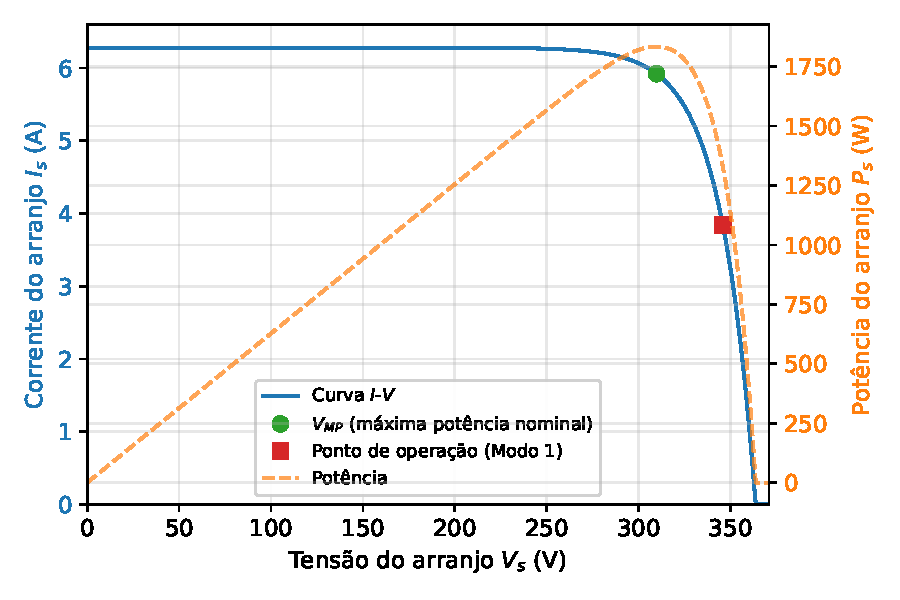
\includegraphics[width=\linewidth]{Figuras/curva_iv_pv.pdf}
\caption{Curva $I$-$V$ e de potência do arranjo fotovoltaico
($N_{s,mod}=17$, $N_{p,mod}=2$), com a tensão de máxima potência nominal
($V_{MP}$) e o ponto de operação autoconsistente do Modo~1 destacados.}
\label{fig:curva_iv_pv}
\end{figure}

\begin{figure}[h]
\centering
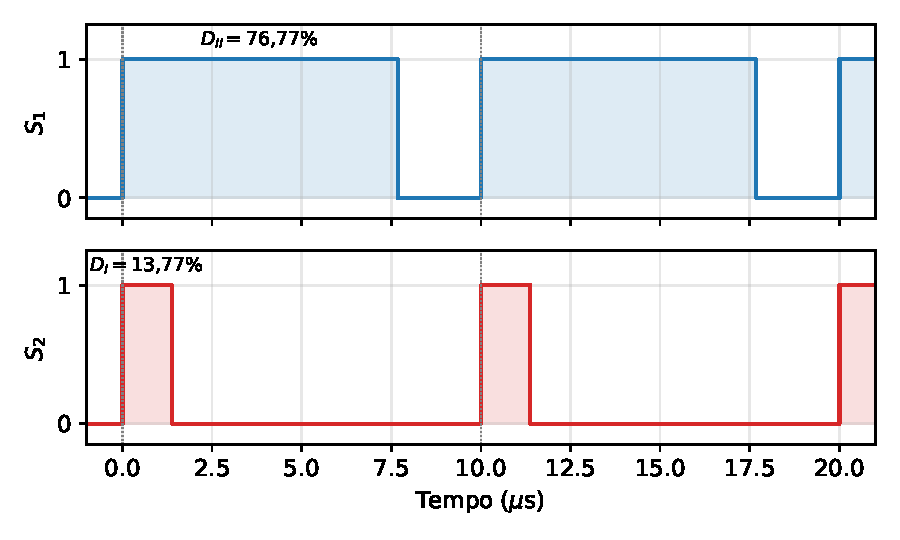
\includegraphics[width=\linewidth]{Figuras/pwm_pulsos.pdf}
\caption{Sinais de comutação de $S_1$ e $S_2$ dentro de um período de
comutação $T_{sw}=10\,\mu\text{s}$, com $S_2$ (duração $D_i$) contido no
intervalo de fechamento de $S_1$ (duração $D_{ii}$), ambos iniciando em
$t=0$.}
\label{fig:pwm_pulsos}
\end{figure}

\subsection{Modelagem do Painel Fotovoltaico}
\label{subsec:modelagem_pv_impl}

O painel fotovoltaico foi implementado como um subsistema mascarado
combinando um bloco \texttt{MATLAB Function} -- que resolve o modelo de
diodo único apresentado na Eq.~\eqref{eq:pvmodel} -- com os componentes
físicos do Simscape responsáveis pela interface elétrica: um sensor de
tensão, que mede $V$ nos terminais do painel e o converte para o domínio de
sinal (\texttt{PS-Simulink Converter}); e uma fonte de corrente controlada
(\texttt{Controlled Current Source}), que injeta a corrente calculada $I$
de volta ao circuito físico após a conversão inversa
(\texttt{Simulink-PS Converter}). Essa arquitetura fecha a malha algébrica
$V \rightarrow I \rightarrow V$ inteiramente no domínio físico do Simscape,
sem necessidade de tratamento explícito de laço algébrico no domínio de
sinal.

Os parâmetros de catálogo adotados correspondem ao painel monocristalino de
\cite{ayaz2014improved} ($I_{SC,ref}=3{,}14$~A, $V_{OC,ref}=21{,}4$~V,
$N_s=36$ células), complementados por coeficientes de temperatura típicos
de painéis dessa classe ($K_v=-0{,}080$~V/°C, $K_i=0{,}0024$~A/°C), uma vez
que esses coeficientes não constam no artigo de referência. As entradas de
irradiância ($G$) e temperatura ($T$) são fornecidas por blocos
\texttt{Stair Generator}, permitindo a aplicação de degraus que emulam
variações de nebulosidade e temperatura ambiente durante a simulação. O
bloco mascarado permite ainda configurar a associação série/paralelo do
arranjo, por meio dos parâmetros $N_{s,mod}$ (módulos em série) e
$N_{p,mod}$ (fileiras em paralelo), escalando a tensão de circuito aberto e
a corrente de curto-circuito equivalentes do arranjo, respectivamente.

\subsection{Modelagem da Bateria}
\label{subsec:modelagem_bat_impl}

O banco de baterias foi modelado segundo o modelo dinâmico genérico de
Shepherd, na formulação proposta por \cite{tremblay2007generic}, amplamente
utilizado em simulações de sistemas híbridos e veiculares. A tensão de
circuito aberto é dada por

\begin{equation}
E = E_0 - K\frac{Q}{Q - it}\,it + A\,e^{-B\cdot it},
\label{eq:battery_ocv}
\end{equation}

em que $E_0$ é a tensão constante do modelo, $K$ a constante de
polarização, $Q$ a capacidade nominal, $A$ e $B$ os parâmetros da zona
exponencial da curva de descarga, e $it$ a carga já extraída da bateria
(Ah). A tensão nos terminais é então

\begin{equation}
V_{bat} = E - R\,I_{bat},
\label{eq:battery_terminal}
\end{equation}

onde $R$ é a resistência interna e $I_{bat}$ a corrente da bateria
(convenção positiva para descarga). A variável $it$ não é calculada
internamente ao bloco \texttt{MATLAB Function}, por se tratar de uma
grandeza dinâmica: ela é obtida por um bloco \texttt{Integrator} externo,
que integra $I_{bat}/3600$ ao longo do tempo, com condição inicial
$it_0 = Q\,(1 - SOC_0/100)$ correspondente ao estado de carga inicial
desejado. O estado de carga percentual é obtido por
$SOC = 100\,(1 - it/Q)$.

A corrente de bateria $I_{bat}$ é limitada por um resistor série cujo valor
cresce proporcionalmente ao excesso de corrente em relação a um limiar de
referência -- distinto para carga ($0{,}5\text{C}$, $1{,}15$~A) e descarga
($2\text{C}$, $4{,}6$~A) --, de modo que a corrente de regime pode assentar
acima do limiar nominal quando há potência excedente disponível no
arranjo fotovoltaico, sem que ocorra um corte abrupto de corrente.

De forma análoga ao painel fotovoltaico, a interface elétrica do subsistema
da bateria é composta por um sensor de corrente (medindo $I_{bat}$ em
série com o ramo) e uma fonte de tensão controlada
(\texttt{Controlled Voltage Source}), que aplica $V_{bat}$ calculado pela
Eq.~\eqref{eq:battery_terminal} de volta ao circuito físico.

Os parâmetros adotados para uma célula/módulo unitário
($E_0=16{,}8$~V, $K=0{,}0076$~V/Ah, $Q=2{,}3$~Ah, $A=0{,}26422$~V,
$B=26{,}5487$~Ah$^{-1}$, $R=0{,}01\,\Omega$) representam um banco de
baterias de íon-lítio genérico, com tensão nominal compatível com a tensão
de bateria considerada em \cite{srinivasa2016vrbess} ($V_{bat}\approx16$~V).
Assim como no painel fotovoltaico, o bloco mascarado do banco de baterias
permite configurar a associação série/paralelo do arranjo por meio dos
parâmetros $N_{s,bat}$ (módulos em série) e $N_{p,bat}$ (ramos em
paralelo), além do estado de carga inicial $SOC_0$.

\subsection{Implementação no Simulink/Simscape}
\label{subsec:implementacao}

Ambos os subsistemas (painel e bateria) seguem o mesmo padrão de
arquitetura: um bloco \texttt{MATLAB Function}, restrito ao domínio de
sinal do Simulink, é acoplado ao domínio físico do Simscape por meio de um
par de conversores (\texttt{PS-Simulink Converter} e
\texttt{Simulink-PS Converter}) e de um componente de medição e um de
atuação física correspondentes -- sensor de tensão e fonte de corrente
controlada no caso do painel; sensor de corrente e fonte de tensão
controlada no caso da bateria. Essa solução foi adotada em substituição aos
blocos pré-construídos de biblioteca (\texttt{PV Array} e \texttt{Battery}
do Simscape Electrical), não disponíveis no ambiente MATLAB Online
utilizado neste trabalho.

Nesta etapa de desenvolvimento, os parâmetros de catálogo de cada
subsistema foram inseridos diretamente no corpo das funções
\texttt{MATLAB Function}, com as entradas dos blocos restritas às
variáveis que efetivamente variam ao longo da simulação -- irradiância
($G$) e temperatura ($T$) no caso do painel, e corrente de bateria
($I_{bat}$) no caso do banco de baterias --, mantendo os demais parâmetros
de catálogo fixos internamente a cada função.

\subsection{Validação em Malha Aberta}
\label{subsec:validacao_ma}

Antes da síntese do controlador FCS-MPC, o conversor VR-BESS e seus
subsistemas de painel fotovoltaico e banco de baterias foram integrados e
validados em malha aberta, com o objetivo de verificar a correta
integração entre os blocos mascarados próprios (Seções~\ref{subsec:modelagem_pv_impl}
e~\ref{subsec:modelagem_bat_impl}) e o domínio físico do Simscape antes da
introdução da malha de controle.

\begin{figure}[h]
\centering
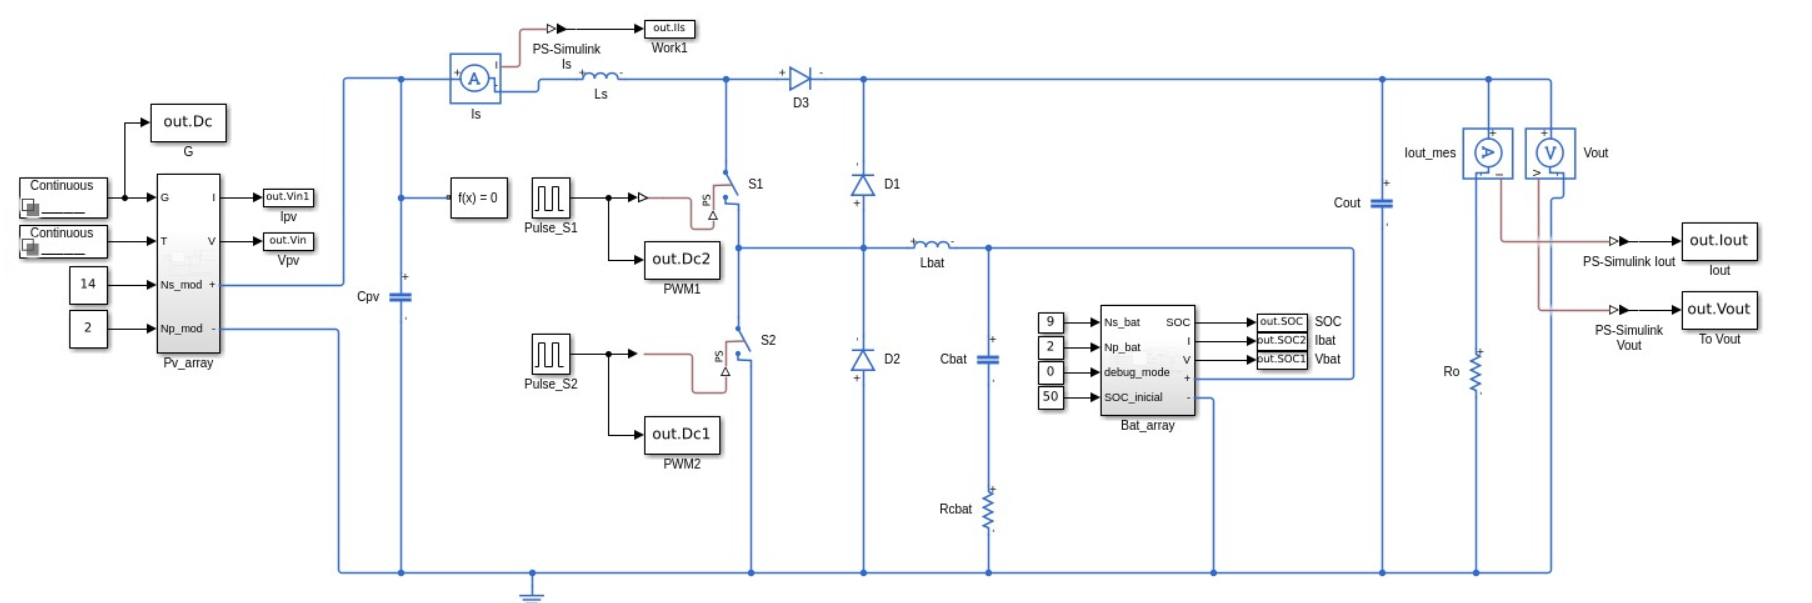
\includegraphics[width=\linewidth]{Figuras/vrbess_simulink_implementado.png}
\caption{Diagrama do modelo VR-BESS implementado no Simulink/Simscape
Electrical, incluindo os subsistemas mascarados de painel fotovoltaico
(\texttt{Pv\_array}) e banco de baterias (\texttt{Bat\_array}) e os
geradores de pulso (\texttt{Pulse\_S1}, \texttt{Pulse\_S2}) utilizados na
validação em malha aberta.}
\label{fig:simulink_implementado}
\end{figure}

Nessa configuração, as chaves $S_1$ e $S_2$ foram acionadas por geradores
de pulso independentes, com razão cíclica fixa dada pela
Eq.~\eqref{eq:duty_valores} e comutação em $f_{sw}=1/T_{sw}=100$~kHz
($T_{sw}=10\,\mu\text{s}$): $S_2$ com razão cíclica de $13{,}77\%$
($1{,}38\,\mu\text{s}$) e $S_1$ com razão cíclica de $76{,}77\%$
($7{,}68\,\mu\text{s}$), ambas com defasagem nula em relação ao início do
período de comutação. O painel fotovoltaico foi configurado com
$N_{s,mod}=17$ módulos em série e $N_{p,mod}=2$ fileiras em paralelo, sob
condição padrão de teste constante ($G=1000\,\text{W/m}^2$,
$T=25\,^{\circ}\text{C}$). O banco de baterias foi configurado com
$N_{s,bat}=15$ módulos em série e $N_{p,bat}=1$ ramo, partindo de um
estado de carga inicial $SOC_0=50\%$, com corrente de carregamento
limitada a $0{,}5\text{C}$ ($1{,}15$~A) e de descarga a $2\text{C}$
($4{,}6$~A). A carga foi fixada em $R_o=160\,\Omega$. Devido à largura
reduzida do pulso de $S_2$ frente ao passo de um solver de passo variável
padrão, adotou-se o \textit{Local Solver} do Simscape (Backward Euler,
passo fixo de $200$~ns) na rede física do conversor. A simulação foi
conduzida por $60$~ms, com as grandezas do domínio físico (tensões e
correntes medidas por sensor) registradas a $T_s=200$~ns. Os resultados
dessa validação são apresentados na Seção~\ref{sec:resultados}.

\section{Resultados}
\label{sec:resultados}

Esta seção apresenta os resultados da validação em malha aberta do
conversor VR-BESS, conduzida conforme os parâmetros descritos na
Seção~\ref{subsec:validacao_ma}: chaves $S_2$ e $S_1$ acionadas por
geradores de pulso independentes com razão cíclica fixa de $13{,}77\%$ e
$76{,}77\%$, respectivamente, comutando a $100$~kHz, sob irradiância e
temperatura constantes ($G=1000\,\text{W/m}^2$, $T=25\,^{\circ}\text{C}$).
O objetivo desta etapa não é avaliar desempenho de controle -- ainda não
implementado --, mas verificar a integração correta entre os subsistemas
de painel fotovoltaico e banco de baterias e o domínio físico do
conversor no Simscape Electrical, além de validar a razão cíclica
recalculada a partir do ponto de operação autoconsistente do arranjo
(Seção~\ref{subsec:duty_cycle}).

Na porta fotovoltaica, configurada com $N_{s,mod}=17$ e $N_{p,mod}=2$, a
corrente do arranjo ($I_{pv}$) apresentou um pico transitório de
$6{,}28$~A -- correspondente a $N_{p,mod}\times I_{SC,ref}=2\times3{,}14$~A
-- durante a energização, estabilizando-se em regime permanente em
$3{,}842$~A. A tensão do arranjo ($V_{pv}$) convergiu, com sobressinal
desprezível, para $345{,}95$~V, valor consistente com o ponto de operação
autoconsistente previsto na Seção~\ref{subsec:duty_cycle}
($V_s\approx344{,}90$~V, erro de $\approx0{,}3\%$), confirmando que a
tensão de regime do arranjo é corretamente determinada pela corrente
demandada pelo conversor, e não apenas pela associação série/paralelo
adotada.

\begin{figure}[h]
\centering
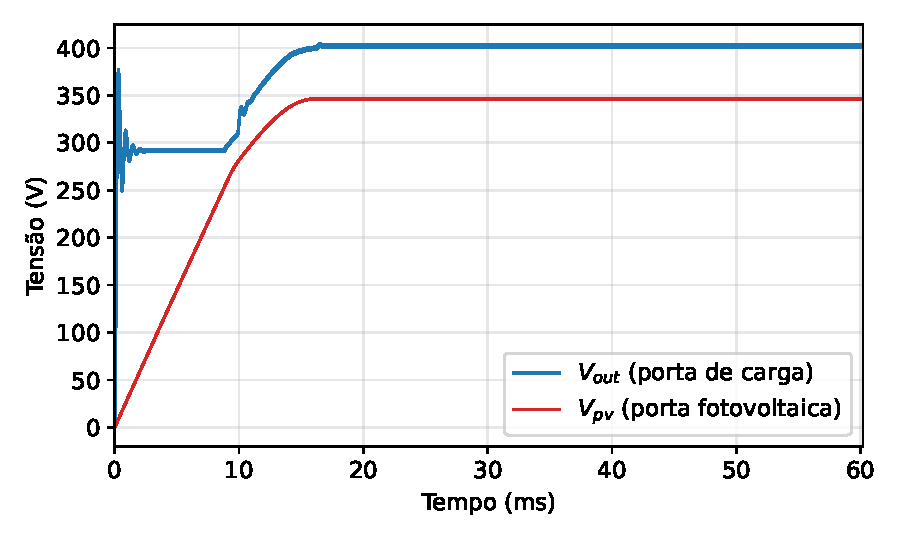
\includegraphics[width=\linewidth]{Figuras/resultado_vpv_vout.pdf}
\caption{Resposta transitória das tensões da porta fotovoltaica ($V_{pv}$)
e da porta de carga ($V_{out}$) sob comutação em malha aberta.}
\label{fig:resultado_vpv_vout}
\end{figure}

Na porta de saída, a tensão sobre a carga ($V_{out}$) convergiu, com pico
de $404{,}24$~V em $t\approx16{,}5$~ms (sobressinal de apenas
$\approx0{,}65\%$ em relação ao valor de regime), para
$401{,}62$~V, com ripple de comutação de $2{,}50$~V pico-a-pico
($\approx0{,}62\%$). Esse resultado corresponde a um desvio de apenas
$\approx0{,}4\%$ em relação à tensão de projeto de $400$~V, validando a
razão cíclica recalculada a partir do ponto de operação autoconsistente do
arranjo (Seção~\ref{subsec:duty_cycle}), em contraste com o desvio muito
maior obtido ao se utilizar a razão cíclica calculada a partir da tensão
de máxima potência nominal do arranjo (Seção~\ref{subsec:duty_cycle}). A
relação ideal de ganho do estágio Boost também se confirma:
$V_o=V_{pv}/(1-D_i)=345{,}95/0{,}8623\approx401{,}2$~V, contra os
$401{,}62$~V medidos (erro de $\approx0{,}1\%$). A corrente de carga
($I_{out}$) se estabeleceu em $2{,}510$~A, resultando em
$R_o=V_{out}/I_{out}\approx160{,}0\,\Omega$, consistente com o valor
resistivo adotado.

Na porta de armazenamento, configurada com $N_{s,bat}=15$, $N_{p,bat}=1$ e
estado de carga inicial $SOC_0=50\%$, a tensão de bateria ($V_{bat}$)
manteve-se praticamente constante em $251{,}92$~V, compatível com a tensão
em circuito aberto esperada para o arranjo
($N_{s,bat}\times E_0=15\times16{,}8=252$~V) na vizinhança de
$SOC=50\%$. A corrente de bateria ($I_{bat}$) apresentou um transitório
inicial de até $5{,}48$~A antes de se estabilizar em um valor médio de
regime de $\approx-1{,}23$~A -- negativo, na convenção positiva para
descarga adotada na Eq.~\eqref{eq:battery_terminal}, indicando
carregamento --, com ripple de comutação de $\approx0{,}037$~A
pico-a-pico. Esse valor situa-se $\approx7\%$ acima do limiar de
$0{,}5\text{C}$ ($1{,}15$~A) adotado para a corrente de carregamento,
consistente com a natureza do limitador proporcional implementado no
modelo da bateria (Seção~\ref{subsec:modelagem_bat_impl}), que permite à
corrente de regime assentar próxima ao limiar nominal sem impor um corte
abrupto. O estado de carga (SOC) permaneceu praticamente inalterado
($50{,}0004\%$) no intervalo analisado, compatível com a baixa taxa de
carregamento frente à capacidade do banco.

\begin{figure}[h]
\centering
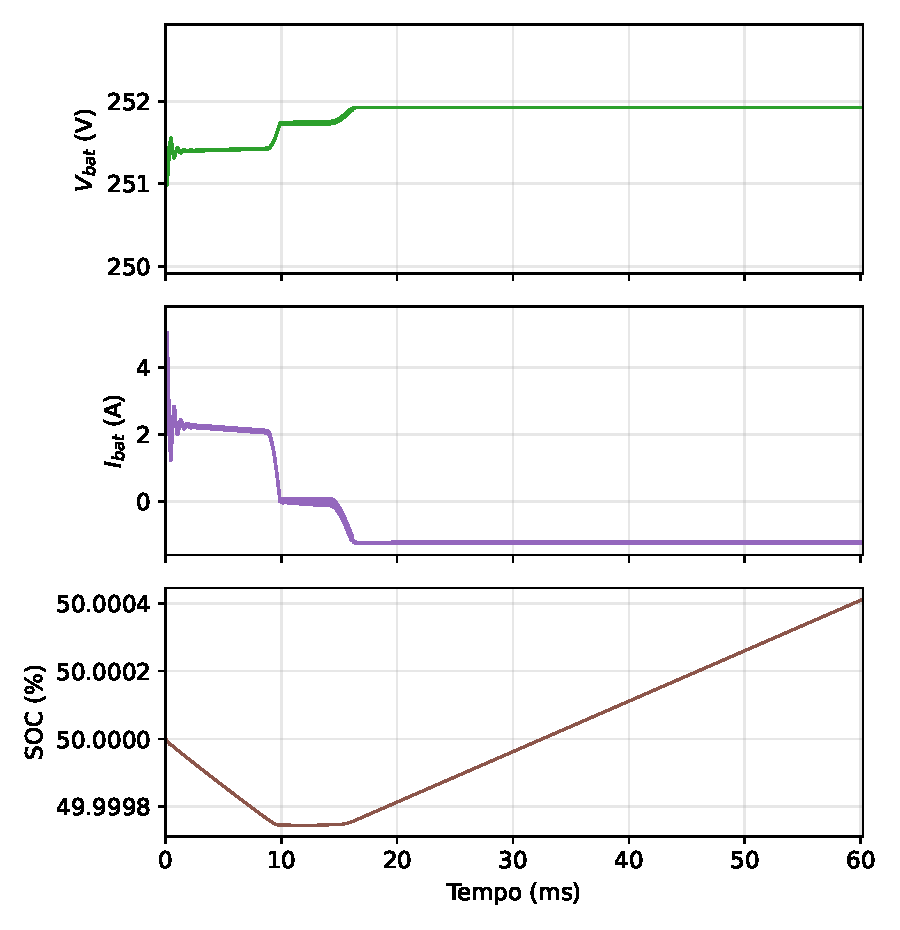
\includegraphics[width=\linewidth]{Figuras/resultado_bateria.pdf}
\caption{Tensão de bateria ($V_{bat}$), corrente de bateria ($I_{bat}$) e
estado de carga (SOC) da porta de armazenamento.}
\label{fig:resultado_bateria}
\end{figure}

Por fim, a corrente no indutor compartilhado da porta fotovoltaica
($I_s$), medida diretamente no ramo comutado, acompanhou a corrente do
arranjo $I_{pv}$ em regime ($\approx3{,}842$~A, ripple de $0{,}125$~A
pico-a-pico), com uma excursão transitória negativa de até $-0{,}60$~A
durante a energização do conversor, compatível com o comportamento
esperado de um indutor submetido a comutação dura em malha aberta.

Em conjunto, esses resultados confirmam a integração correta entre os
blocos mascarados de painel fotovoltaico e banco de baterias e o domínio
físico do conversor VR-BESS, com a tensão de saída convergindo para
próximo do valor de projeto ($401{,}62$~V frente aos $400$~V especificados)
a partir da razão cíclica recalculada pelo método de ponto fixo
apresentado na Seção~\ref{subsec:duty_cycle}. Essa validação confirma que,
diferentemente da tensão de bateria -- fixada essencialmente pela
associação série do banco --, a tensão do arranjo fotovoltaico em regime é
determinada pela corrente demandada pelo conversor, exigindo o cálculo da
razão cíclica a partir do ponto de operação autoconsistente do arranjo, e
não da tensão de máxima potência nominal. Essa validação em malha aberta
estabelece a base de simulação sobre a qual o controlador FCS-MPC,
apresentado na Seção~\ref{subsec:fcsmpc}, será implementado e avaliado --
em substituição aos geradores de pulso de razão cíclica fixa por uma lei
de comutação em tempo real capaz de manter $V_{out}$ regulado mesmo
quando a corrente de carregamento da bateria variar em relação ao ponto
de operação aqui calibrado -- na etapa subsequente deste trabalho.

\section{Conclusão}
\label{sec:conclusao}

Este trabalho apresentou o desenvolvimento do conversor CC-CC de três
portas do tipo VR-BESS para integração de painel fotovoltaico, banco de
baterias e carga, com vistas à futura aplicação da técnica FCS-MPC. Foram
implementados, como blocos mascarados próprios em substituição às
bibliotecas nativas do Simscape Electrical (indisponíveis no ambiente
MATLAB Online utilizado), os modelos do painel fotovoltaico de diodo único
e da bateria de íon-lítio segundo a formulação de Shepherd, integrados ao
domínio físico do conversor por meio de sensores e fontes controladas.

A validação em malha aberta, conduzida com as chaves sob razão cíclica
fixa, confirmou a correta integração entre esses subsistemas e o
conversor: as grandezas de regime permanente observadas em cada porta --
corrente do arranjo fotovoltaico, tensão e corrente de bateria, estado de
carga e tensão de saída -- mostraram-se coerentes com os parâmetros de
projeto adotados (configuração série/paralelo dos arranjos, parâmetros de
catálogo do painel e da bateria), inclusive quanto à variação do estado de
carga frente à corrente de bateria integrada. Esses resultados consolidam
a base de simulação -- planta, sensores e atuadores no domínio físico --
sobre a qual o controlador será desenvolvido.

A validação também evidenciou que a tensão do arranjo fotovoltaico em
regime depende da corrente demandada pelo conversor -- e não apenas da
associação série/paralelo adotada --, de modo que a razão cíclica de
$S_2$ precisou ser calculada a partir do ponto de operação
autoconsistente do arranjo sob a corrente do Modo~1
(Seção~\ref{subsec:duty_cycle}), e não a partir da tensão de máxima
potência nominal. Essa calibração é válida para a corrente de
carregamento de bateria observada nesta validação; variações nessa
corrente -- decorrentes, por exemplo, da evolução do estado de carga da
bateria ou de mudanças na irradiância -- deslocam o ponto de operação e
exigiriam uma nova calibração da razão cíclica, o que reforça a
necessidade do controlador em malha fechada proposto para a etapa
subsequente do trabalho.

O trabalho não abrangeu, até o momento, a implementação da malha de
controle: os resultados aqui apresentados refletem o comportamento do
conversor sob comutação em malha aberta, sem regulação ativa de tensão de
saída ou de corrente de bateria, e para um único ponto de operação, sem
degraus de irradiância, carga ou referência. A etapa subsequente deste
trabalho consiste em implementar o controlador FCS-MPC descrito na
Seção~\ref{subsec:fcsmpc} sobre a planta validada, avaliando sua capacidade
de regulação da tensão de saída e de gerenciamento da corrente de bateria
frente a esses cenários, bem como investigar o emprego dos observadores de
estado apresentados na Seção~\ref{subsec:observadores} como alternativa
para redução do número de sensores físicos necessários à implementação do
controlador.


%===============================================================================
% REFERÊNCIAS
%===============================================================================
\bibliography{ifacconf}

\end{document}
